% +------------------------------------------------------------------------+
% | CGAL Reference Manual:  Box_intersection_d/main.tex
% +------------------------------------------------------------------------+
% | Fast iso-box intersections
% |
% | 2003, 2004   Lutz Kettner, Andreas Meyer, Afra Zomorodian
% | 
\RCSdef{\BoxIntersectionRev}{$Revision$}
\RCSdefDate{\BoxIntersectionDate}{$Date$}
% +------------------------------------------------------------------------+

\newcommand{\LK}[1]{\textbf{L.K.:#1???}}

\ccParDims

\chapter{Intersecting Sequences of Iso-oriented Boxes}
\label{chapterBoxIntersection}
\ccChapterRelease{\BoxIntersectionRev. \ \BoxIntersectionDate}\\
\ccChapterAuthor{Lutz Kettner, Andreas Meyer, and Afra Zomorodian}


% +------------------------------------------------------------------------+
\section{Introduction}

We provide an efficient algorithm~\cite{cgal:ze-fsbi-02} for finding all
intersecting pairs for large numbers of iso-oriented boxes, i.e.,
typically these will be bounding boxes of more complicated geometries.

Computing information about complex geometric primitives is often
expensive. While researchers in computational geometry have discovered
many asymptotically efficient algorithms for such problems, the
algorithms are often of theoretical interest only, as they are hard to
implement or slow if implemented. One general approach is to reduce
the problem size enough so that a brute force method is feasible and
fast. By putting axis-aligned bounding boxes around complicated
primitives, we can compute, in a short amount of time, an approximate
answer in the form of a small set of pairs with potential interaction.
We then refine our answer by looking inside the boxes, computing the
exact answer for the original data.

Many geometric problems can be restated in terms of box intersections
since if the bounding boxes of two primitives intersect, we know that
the primitives may intersect or have close proximity. Some practical
problems we may solve with this approach include detecting surface
self-intersection, intersection of two different objects and
performing proximity queries.


% +------------------------------------------------------------------------+
\section{Iso-oriented Box}

The iso-oriented box, or bounding box, can have arbitrary dimension.
An interval specifies the size of the box in each dimension. The
number type used to represent the interval boundaries is a template
parameter of the box. Useful instantiations are with the builtin
\texttt{int}, \texttt{unsigned int}, \texttt{double} or \texttt{float}
types.

We offer two topological interpretations of the box; it can be a
half-open set or a closed set. The box is half open if its intervals
$[lo_i,hi_i)$ are half open in each dimension $i$. Analogously, a box
is closed if its intervals $[lo_i,hi_i]$ are closed in each dimension
$i$. Note that closed boxes support zero-width boxes and they can
intersect at their boundaries, while half-open boxes always have a
positive volume and they only intersect iff their interiors overlap.
The distinction between closed or half-open boxes does not require a
different representation of boxes, just a different interpretation
when comparing boxes. This is handled flexible inside the traits class
parameter passed to the intersection algorithm.

We need an arbitrary fixed order on the boxes to guarantee that a pair
of intersecting boxes is reported only once in the algorithm, in
particular, this is needed for the self-intersection test, i.e., when
we use the algorithm to find all intersections in one set of boxes. In
that case we need a second copy of the boxes that is distinguishable
from the first set of boxes. We can achieve the fixed order, for
example, by assigning unique numbers to each box. Assuming boxes are
allocated at distinct memory locations we can use their memory address
to define such unique numbers. However, that does not suffice in the
self-intersection case where we would need an explicit second copy to
get distinct memory addresses.

We offer a default iso-oriented box type that
\begin{itemize}
  \item implements a standard bounding box,
  \item is generic in terms of number type and dimension: \\
  \texttt{template< class T, unsigned int DIM > struct Default\_box\_d},
  \item provides an explicit unique numbering, and
  \item can be used as a base class to derive a user defined box with
  additional information, for example, the exact geometry
  that was approximated with the bounding box.
\end{itemize}

We require the box type to be assignable. Everything else is 
factored into the following traits class.

% +------------------------------------------------------------------------+
\section{Traits Class for Iso-oriented Box}

The access to the iso-oriented box is exclusively done using a 
traits class, which serves as an adaptor. This adaptor hides the
specific interface a box may have. As an example, we show the
implementation of the default traits class for the
\texttt{Default\_box\_d}:

\begin{ccExampleCode}
template< class Box_ >
struct Default_box_traits_d {
    typedef const Box_&       Box;
    typedef typename Box_::NT NT;

    static NT          get_lo( Box b, std::size_t dim) { return b.get_lo(dim);  }
    static NT          get_hi( Box b, std::size_t dim) { return b.get_hi(dim);  }
    static std::size_t get_id( Box b)                  { return b.get_id();     }
    static std::size_t get_dim()                       { return Box_::get_dim();}
};
\end{ccExampleCode}

This default traits class can be used for our \texttt{Default\_box\_d}
or box classes derived from it. Therefore its chosen as default for
the box intersection algorithm. If a different custom box class is
used, the user has to provide a suitable traits class.

The requirements for the \ccc{BoxTraits_d} concept are:
\begin{itemize}
    \item 
      \texttt{Box} is the box type used in passing box objects to the
      functions.\LK{Why is const-ref part of Box}
    \item
      \texttt{NT} is the number type used for the interval
      boundaries. It must support all comparison operators.
      \LK{How about construction of min/max-inf}
    \item 
      \texttt{get\_lo} and \texttt{get\_hi} return the low and high
      interval boundaries of the corresponding dimension argument
      \texttt{dim}, where the first  dimension has the index zero.
    \item 
      \texttt{get\_num} returns the unique number of that box. The
      return type is not required to be \texttt{std::size\_t}. Any
      type supporting \texttt{==} and \texttt{<} operators for a total
      order suffice.
    \item
      \texttt{get\_dim} returns the number of dimensions. 
\end{itemize}

\begin{ccAdvanced}
  A more detailed interface is provided with the box predicate traits
  class. It implements the various predicates used in the box
  intersection algorithm. It is exchangeable and can be used by
  experts to fine tune the comparisons performed in this algorithm,
  e.g. utilizing machine instruction sets, see the
  \ccc{BoxPredicateTraits_d} concept in the reference manual section
  for more details. Note that the generic default model provided is
  fully functional and efficient in all cases, thus usually there is
  no need to look at this predicate traits. 
\end{ccAdvanced}



% +------------------------------------------------------------------------+
\section{Intersection Algorithm}

The conventional application of this algorithm will start from 

First, for each geometric primitive, a bounding box has to be
computed. Any bounding box class can be used, as long as a box adaptor
exists for it. The bounding box sets have to be supplied to the
algorithm by pairs of \ccc{Random Access Iterators}. While checking,
each bounding box intersection is written to an output iterator as two
boxes. The input box sets need not be sorted in any order.

If the used box class is derived from the default bounding box (or at
least has the same fields), there is no need to specify a box adaptor.
When no box adaptor is given, it is assumed that the default box
adaptor can be used to access the supplied boxes. A minimal example
using just the defaults demonstrates the invocation:

\ccIncludeExampleCode{Box_intersection_d/minimal.C}

Here, the box type is exactly the default box using three dimensions
and \texttt{double} as the underlying number type. A number of boxes
is filled with random data and all box intersections are reported as
pairs of numbers. The callback has to accept two boxes of type similar
to the iterator's value type.

Notice that the default box adaptor is a template with a box type
argument. The box type needed for the adaptor is infered from the
iterator's value type. It may be a class type or a pointer to a class.
Default box traits templates exist for both kinds of types.

It may be surprising, but here using plain structures instead of
pointers to boxes is actually faster. Copying pointers is of course
much faster than copying a whole structure, which may be eight times
larger. But accessing a set of structures is faster when they are
grouped together, so that the range of memory already cached in some
way. While processing, the boxes are sorted and partitioned so that
cacheing becomes effective. Of course, if the used hardware has no
cache capabilities at all, there is no point in prefering plain
structures against pointers.

% \subsubsection*{Performance Parameters}

Internally, the bounding box check uses a streamed segment tree. A
cutoff threshold parameter specifies the minimum amount of boxes so
that the segment tree is used. Below this minimum, a simpler algorithm
is used that has less overhead and performs well only for low number
of boxes and dimension. The choice of a cutoff parameter can have a
significant effect on runtime. If the cutoff value is near to the
overall number of boxes, the runtime may in extreme cases equal that
of the simpler algorithm because it is invoked too early. Threshold
values that are too low invoke the simpler algorithm too late and add
some unneccessary overhead to the overall runtime.

Unfortunately, there is no general method to automatically determine
an optimal cutoff parameter, since it depends on the used hardware,
the callback runtime/segment tree runtime ratio and of course the
number of boxes to be checked. In cases where the callback runtime is
dominant, it may be best to set the threshold parameter to values near
zero. Otherwise a formula like $cutoff=\sqrt{n}$ can lead to
acceptable results. However, for optimal runtime some experiments to
compare different cutoff parameters are required.

In general:

\begin{itemize}
    \item
      When using a reasonable cutoff parameter, the runtime is
      $O((n+m)\log^{d}(n+m)+k)$, where $n$ and $m$ are the number of
      boxes, $d$ is number of dimensions (starting with one) and $k$
      is number of box intersections. 
    \item
      In cases of a badly chosen cutoff parameter, the runtime drops
      to $O(n\log n+m\log m+k`)$ where $k`$ is the number of
      intersections of a one dimensional interval set in which for
      each box in the box set, only the interval in dimension $d$ is
      considered. If all boxes are arranged in a row, so that in
      dimension $d$ all intervals overlap, $k`=n*m$ which is much
      higher than the usual $k=O(n+m)$. 
    \item
      Space requirement is $O(n+m)$ for the user provided boxes. No
      new space is allocated while computing.  
\end{itemize}

Of course, in the complete case $n+m$ has to be substituted with $n$.

% +------------------------------------------------------------------------+
\section{Example Programs}

All examples use closed boxes. No cutoff parameter is specified, so
the default of 10 is used.

\subsection{Custom Box}

This shows how to use a custom box, together with the default box
traits. For simplicity, the custom box inherits from the default box.
A primitive field is added. Primitives intersect each other with a
certain fixed probability. The point here is, that the box traits
class need not be specified. If pointers to the custom box were stored
inside the box container, the pointer specialization of the box traits
template is used automatically, with the custom box as the template
parameter.

\ccIncludeExampleCode{Box_intersection_d/custombox.C}

\subsection{Custom Box Traits }

Here, a bounding box is a cube. This saves some space at the expense
of precision. The custom box only contains a vector to the minimal
point plus a size for all three dimensions. The primitive class is the
same as in the custom box example above. Invocation differs only where
the box traits must be supplied as an argument.

\ccIncludeExampleCode{Box_intersection_d/customadaptor.C}

% +------------------------------------------------------------------------+
\section{Implementation}

\cgal{} makes liberal use of exact number types, which often has a
significant impact on performance. Many algorithms depend on the usage
of exact number types. However, the bounding box intersection
presented here only approximates some geometric primitives, and as
such does not rely on exact representation of numbers. An important
consequence is that \ccc{float} and \ccc{double} number types can be
used, which are much faster, also because of hardware implementation.
To demonstrate that box intersection can be done quite fast, different
box sets are intersected in the range between 4 and 800000 boxes.
Here, the size is the sum both set's sizes. Only plain default boxes
are used, without carrying additional data fields. Boxes use closed
topology, are of dimension three and as number type 32 bit
\ccc{floats} are used. All boxes are stored as plain structures, not
as pointers. Hardware used is a Xeon 2.4GHz equipped with 4GB of
memory.

For each box set, a near-optimal cutoff parameter is determined using
an adaptive approximation. The runtime required for streaming is
compared against usual scanning. Each box intersection is reported to
a dummy callback, which itself does nothing. Results can be seen in
figure \ref{fig_benchmark}. As can be seen, for low numbers of boxes,
pure scanning is still faster than streaming with optimal cutoff,
which would just delegate the box sets to the scanning algorithm. As
there are more and more boxes, the overhead becomes less important.

\begin{ccTexOnly}
 \begin{figure}
  \begin{center}
  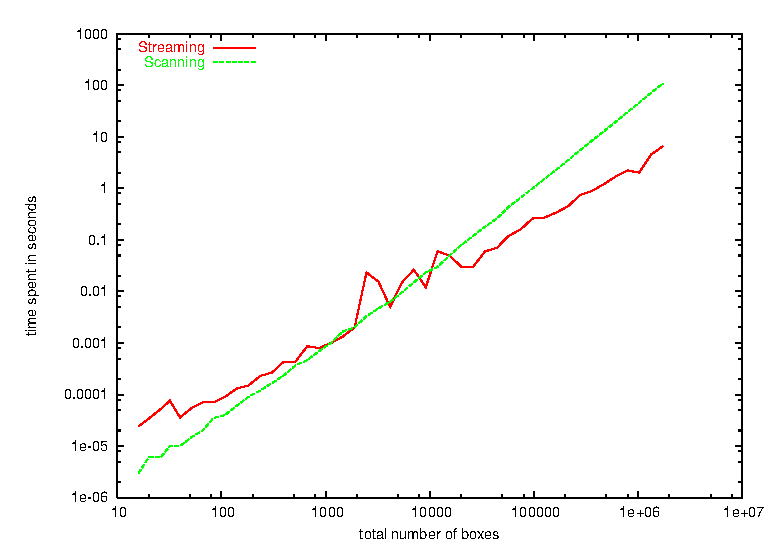
\includegraphics[width=0.5\textwidth]{Box_intersection_d/fig/benchmark}
  \caption{Runtime comparison scanning vs. streaming.}
  \label{fig_benchmark}
  \end{center}
 \end{figure}
\end{ccTexOnly}



%% EOF %%
